% TODO: Add n.d. as year entry for bib entries that don't have a date. (Search for "()" in the PDF)

\documentclass{article}
\usepackage[hidelinks]{hyperref}
\usepackage{csquotes}
\usepackage[vmargin=25mm, hmargin=20mm]{geometry}
\usepackage{xcolor}
\usepackage{graphicx}
\usepackage{float}
\usepackage{listings}
\lstset{
    backgroundcolor=\color[RGB]{240, 240, 240},   
    basicstyle=\ttfamily,
    breakatwhitespace=false,
    breaklines=true,
    keepspaces=true,
    numbers=left,
    numbersep=5pt,
    showspaces=false,
    showstringspaces=false,
    showtabs=false,
    tabsize=4,
    postbreak=\mbox{\textcolor{red}{$\hookrightarrow$}\space}
}
\usepackage[
    backend=biber,
    sorting=none,
    style=ieee,
    urldate=long,
    maxcitenames=2,
    mincitenames=1
]{biblatex}
\addbibresource{sources.bib}
\usepackage{multicol}
\setlength{\columnsep}{13mm}
\usepackage{caption}
\captionsetup{justification=centerlast,font=small,labelfont=sc,margin=50pt}


\title{%
\vspace{50px}%
    \Huge Differential Fuzzing on coreutils Using LibAFL\break%
    —\break%
    Report%
    \vspace{250px}%
}

\author{%
  Valentin Huber\vspace{5px}\\%
  \small \href{https://www.zhaw.ch/en/engineering/institutes-centres/init/}{Institute of Applied Information Technology}\\%
  \small \href{https://www.zhaw.ch/en}{Zürich University of Applied Sciences ZHAW}\\%
  \small \href{mailto://contact@valentinhuber.me}{contact@valentinhuber.me}%
  \vspace{10px}
}
\date{\today\vspace{5px}}

\DeclareFieldFormat*{citetitle}{\textit{#1}}
\hfuzz=50px
\hbadness=10000
\newcommand{\code}[2][]{\lstinline[language=#1, breaklines=false]{#2}}
\let\savedCite=\cite
\renewcommand{\cite}{\unskip~\savedCite}
\let\savedRef=\ref
\renewcommand{\ref}{\unskip~\savedRef}

\begin{document}
\pagenumbering{gobble}
\maketitle

\clearpage\newpage
\begin{center}
    \begin{minipage}{0.8\textwidth}
        \vspace{70px}
        \begin{abstract}
            Hello, %
            %
            World!
        \end{abstract}
    \end{minipage}
\end{center}

\clearpage\newpage
\newgeometry{vmargin=25mm, hmargin=40mm}
\tableofcontents
\clearpage\newpage
\restoregeometry
\pagenumbering{arabic}

\begin{multicols}{2}
    \section{Introduction}
    \subsection{Differential Fuzzing}
    \begin{itemize}
        \item Fuzzing has been popular and effective at finding bugs.
        \item Much research has gone into input selection/guiding.
        \item Not much has been done when it comes to oracles.
        \item Differential Fuzzing: What it is.
    \end{itemize}

    \subsection{coreutils}
    \begin{itemize}
        \item Short overview
        \item uutils' version
    \end{itemize}

    \subsection{LibAFL}
    \label{LibAFLHistory}
    \begin{itemize}
        \item History of AFL/AFL++
        \item Problems with incompatible forks and how LibAFL attempts to fix them
    \end{itemize}

    \subsection{Research Questions}
    \begin{enumerate}
        \item Which parts of coreutils can be fuzzed? What performance tradeoffs does each part introduce?
        \item How can the necessary instrumentation be introduced into coreutils? What are the engineering and performance implications of each option?
        \item Can LibAFL feasibly be used to build a system with all logic defined in the answers to the questions above?
        \item If yes, how effective is the resulting fuzzer at finding bugs in coreutils? What kind of bug can be found with it?
        \item Can the system be expanded to implement differential fuzzing between the different implementations? What changes are necessary?
        \item If yes, how effective is the this second fuzzer at finding bugs in coreutils? What kind of bug can be found with it?
    \end{enumerate}

    \section{Background}
    \subsection{coreutils}

    On \citedate{FileUtilsAnnouncement}, {\DeclareNameAlias{labelname}{given-family}\citeauthor{FileUtilsAnnouncement}} announced fileutils, a suite of utilities for reading and altering files\cite{FileUtilsAnnouncement}. A year later, he released textutils (to parse and manipulate text)\cite{TextUtilsAnnouncement} and shellutils (to write powerful shell scripts)\cite{ShellUtilsAnnouncement}. These three collections were folded into one on \citedate{CoreUtilsAnnouncement}, called the GNU coreutils.\cite{CoreUtilsAnnouncement} \code{ls}, \code{cat}, \code{base64}, \code{grep}, \code{env}, or \code{whoami}: GNU's coreutils are at the basis of how users interact with most Linux distributions on the command line.\cite{GNULinux} Because they are so widely used and central to how users interact with their computers, software quality and lack of software defects is especially important to coreutils.

    Version 9.5 of the GNU coreutils was released on \citedate{GNUCoreUtils9.5} and thus marks the current version as of this report. 106 programs are built per default.\cite{GNUCoreUtils9.5}

    \subsubsection{Interface}
    \label{CoreutilsInterface}

    Users primarily interact with coreutils through the command line or in shell scripts. They take different kinds of inputs, i.e. behave differently based on changes to:
    \begin{itemize}
        \item Data passed to \code{stdin}, e.g. through Unix pipes
        \item Command line arguments:
              \begin{itemize}
                  \item Unnamed arguments, either required (such as \code{cp <source> <destination>}) or optional (such as \code{ls [directory]})
                  \item Flags without any associated data, such as \code{--help}
                  \item Flags with associated data, either required (such as \code{dd if=<input file> of=<output file>}) or optional {such as \code{-name <pattern>} in \code{find}}
              \end{itemize}
        \item Environment variables, such as \code{LANG}
        \item The file system content, such as for \code{ls}
    \end{itemize}

    The output, or effects of invocations fall into the following categories:
    \begin{itemize}
        \item Data written to \code{stdout}
        \item Data written to \code{stderr}
        \item The exit status of the process
        \item The signal terminating the process
        \item Changes to the file system
    \end{itemize}

    \subsubsection{Alternative Implementations}

    Since the release of GNU coreutils, multiple alternative implementations were released. Notable among those are BusyBox\cite{BusyBox}, which aims to provide most of the GNU coreutils with a focus on resource restrictions. It is therefore primarily used in embedded systems\cite{BusyBox} or tiny distributions such as Alpine Linux\cite{Alpine}.

    In the general push towards rewriting software in memory-safe languages, the uutils project\cite{Uutils} maintains a drop-in replacement implementation of the GNU coreutils written in Rust.\cite{UutilsCoreUtils} It does contain all programs, but is still missing certain options. All differences with GNU's coreutils are treated as bugs. It further aims to not only work on Linux, but is also available for MacOS and Windows.

    \subsubsection{Build System}
    \label{CoreutilsBuildSystem}

    The GNU coreutils employ a complex, multi-step build system, including Autoconf\cite{Autoconf} and Automake\cite{Automake}. Changes to either the code or the build system configuration require a deep understanding of the entire ecosystem to ensure no unintended changes to the resulting binaries are introduced. uutils' version of coreutils relies on cargo as its build system, which make outcomes of changes to the code much more predictable.

    \subsection{LibAFL}
    \label{LibAFLBackground}
    As introduced in Section~\ref{LibAFLHistory}, LibAFL is an extendible framework to build custom fuzzers. What follows is a short introduction to the ideas and parts of LibAFL necessary to understand this project. For a more in-depth look, the authors refer to the original LibAFL paper\cite{LibAFL}.

\end{multicols}
\begin{figure}[htbp]
    \centering
    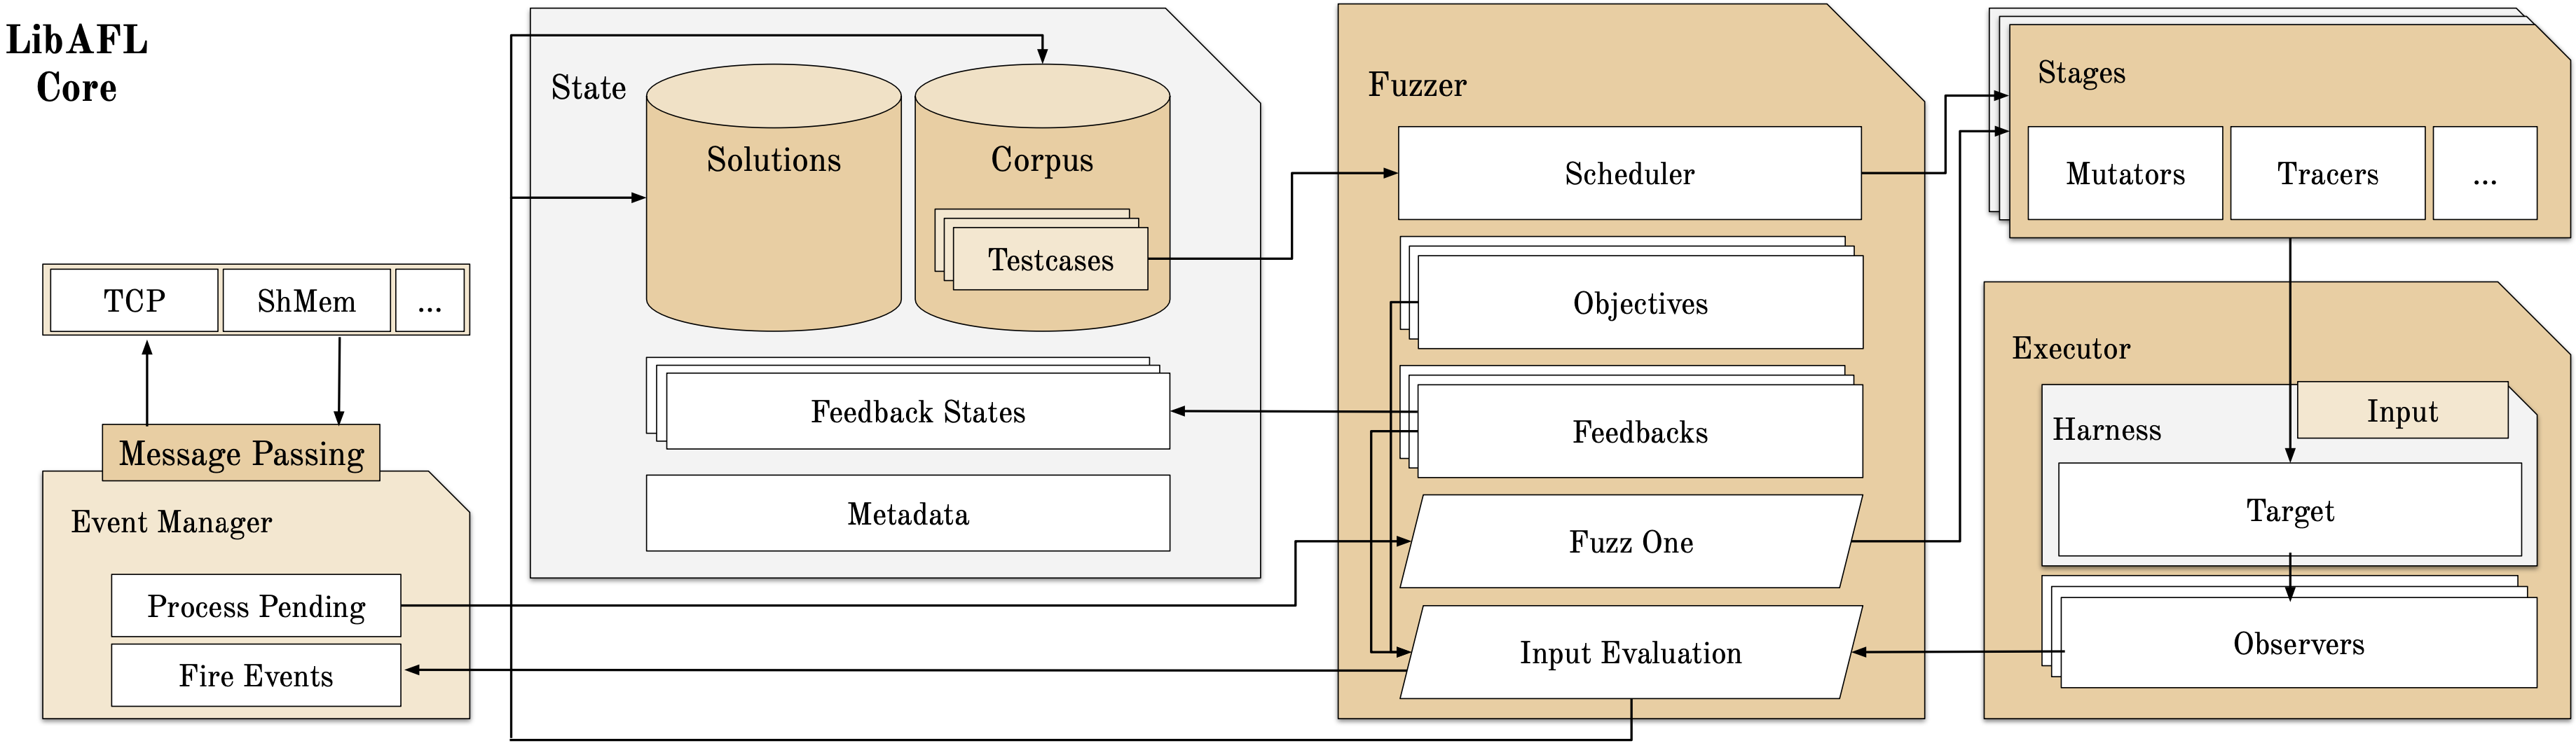
\includegraphics[width=\textwidth]{assets/LibAFLArchitecture.png}
    \caption{LibAFL's Architecture\cite{LibAFL}}
    \label{fig:LibAFLArchitecture}
\end{figure}
\begin{multicols}{2}
    \subsubsection{Generic Concepts}
    The core insight by the authors of LibAFL is that most fuzzers contain very similar parts, where advancements in new works are usually developments in only few of the fundamental fuzzer parts. The logic is usually either introduced into a fork of an existing fuzzer (such as AFL++), which is then abandoned without collecting the advancements in a way that they are reusable and combinable in later projects. Alternatively, authors might elect to create a new system from scratch, which introduces a lot of duplicate work and code, which isn't as optimized as possible, since fuzzer parts such as the thread synchronization usually aren't the focus of new works.

    The authors of LibAFL examined recent innovations in fuzzing and identified a set of distinct parts present in many of the fuzzers. They then designed the architecture of LibAFL in such a way that authors can change just the parts they are interested in and rely on a well-optimized default implementation for everything else. Figure\ref{fig:LibAFLArchitecture} shows the identified fuzzer parts and their interaction, as implemented in LibAFL. Using this architecture, the authors of LibAFL re-implemented the logic introduced in high-impact 20 works to both proof that the system is flexible enough to handle logic created indepen from their system. Finally, they showed that it is now trivial to combine advancements made in different works (i.e. combining the input scheduler of one work with new feedback types introduced in another).

    \subsubsection{Usage of Traits}
    \label{LibAFLTraits}

    On a more technical side, to achieve their goal, the authors heavily relied on Rust's trait system in combination with generic types. This section will present a selection of these core traits, including a short explanation. For a complete list and more expansive documentation, the author refers to the paper which introduced LibAFL\cite{LibAFL} and the official LibAFL book\cite{LibAFLBook}.

    \paragraph{Executor}

    The \code{Executor} is called with a certain \code{Input} and executes the program under test. It ensures that the passed \code{Observer}s can gather whatever information they need to and provide additional information about the execution run. Examples for \code{Executors} include \code{InProcessExecutor}, which calls the provided function directly, \code{InProcessForkExecutor}, which calls \code{fork} before calling the function and trades off additional performance overhead for improved stability. Finally, while being libraries external to the LibAFL core, \code{FridaInProcessExecutor} and \code{QemuExecutor} use the dynamic instrumentation framework Frida resp. the emulator QEMU to support complex fuzzing approaches.

    \paragraph{Observer}

    \code{Observer}s are passed to an \code{Executor} and gather information before, during, or after the execution. This information can take any arbitrary shape. Typical \code{Observer} implementations used in fuzzers include \code{StdMapObserver}, which is often used to keep track of coverage data by recording execution paths, or \code{CmpObserver} to trace comparisons during an execution run.

    \paragraph{Feedback}

    There are two uses for \code{Feedback}s in LibAFL: objectives and feedbacks steering the search. They reduce a combination of information provided by the \code{Executor} and \code{Observer}s to a boolean value: Is this test case interesting? If used as an objective, this marks the test case in question as a solution. If used as a steering feedback, it will add the current test case to the corpus from which (after mutating it) the next input is drawn. Typical examples include a \code{CrashFeedback}, \code{TimeoutFeedback} (both usually used in the objective mode) and a \code{MaxMapFeedback}, which can be used to see if new parts of the memory map used to keep track of the executed parts of the binary are touched, thus representing the coverage-guided part of the fuzzer.

    \paragraph{Input}

    \code{Input}s are about what one would expect: A representation of what is mutated and then passed to the \code{Executor}. Typically, it consists of a simple variable length byte array, but may also be a more complex \code{struct}. Depending on the use case, the former might be sufficient or one might need the additional flexibility provided by the latter.

    \paragraph{Mutator}

    Finally, \code{Mutator}s take an \code{Input} and change it in some form. On simple byte array \code{Input}s, this may be flipping a bit, or injecting an additional byte somewhere. For more complex \code{Input}s, custom \code{Mutator}s may need to be written. All \code{Mutator}s included in a certain fuzzer are passed to a scheduler which mutates an \code{Input} once or multiple times with the received \code{Mutator}s. This is another example of the flexibility of LibAFL: While one may need to write custom \code{Mutator}s for a custom \code{Input} type, all scheduling algorithms available in LibAFL can be used regardless, without any additional changes.

    \section{Implementation}

    This section introduces the concepts and technical details necessary to reproduce the findings of this work by incrementally adding capabilities to a fuzzer. The example fuzzer will target \code{base64}, a comparatively small program from the coreutils. It encodes and decodes binary data to a format consisting only of characters unproblematic in most contexts. It takes its input from either a file or \code{stdin} and provides the following options:
    \begin{itemize}
        \item \code{--decode} switches \code{base64}'s mode from encode to decode
        \item \code{--ignore-garbage} ignores non-alphabet characters when decoding
        \item \code{--wrap <cols>} inserts linebreak after \code{<cols>} characters when encoding
        \item \code{--help} prints information about \code{base64} and exits
        \item \code{--version} prints version information and exits
    \end{itemize}

    \subsection{Basic Unguided Fuzzer}

    The first step is to build a fuzzer without any features: It just takes a byte array, randomly mutates it, feeds it to the fuzzer and checks for crashes. It does not contain any execution steering nor can it trigger the different options. One can choose the default implementations for each part outlined in Section\ref{LibAFLBackground}, which reduces the necessary code for the fuzzer to well under 100 lines. However, this fuzzer is very unlikely to find any software defect, since it essentially employs the same strategy as was proposed in the seminal work by \citeauthor{UNIX} in \citeyear{UNIX}: inserting random data into a program and hoping for a crash, without any additional logic. Additionally, it does not even have access to all parts of the program, since the command line arguments are never used.

    \subsubsection{Environment Protection}
    \label{Environment}

    The most simple solution to allow a fuzzer to access the command line arguments would be to split the byte array at a magic byte (e.g. \code{NULL} bytes), and pass the first entry to \code{stdin} and all remaining as command line arguments. However, this introduces a problem: Some programs in the coreutils can change the environment they are running in, as described in Section~\ref{CoreutilsInterface}. This may be entirely trivial (e.g. creating and writing to a temporary file in an unrelated part of the filesystem), but may also disturb the fuzzing process or even incur irreparable damage to the system by overwriting critical files.

    The fuzzer therefore needs to protect the environment from the effects of the program. This can be done in a few different ways, each of which introduces a certain downside:
    \begin{enumerate}
        \item First, the fuzzer could create a layered filesystem and use it to create an environment for the program under test to run in. This is what Docker uses to use the host's kernel while fooling the program under test into thinking it runs natively. Changes to the file system are captured and stored while read operations are responded to with data from the write layer if it has been changed previously and from the host's file system if not. However, the performance implications of this approach are immense: While starting a coreutils program takes about 20~ms on the author's system, starting a Docker container takes approximately 2~s. Additionally, doing this across many cores, as is typical in modern fuzzing, relies on the parallelization of starting containers as done by the Docker daemon. This is not necessarily the case, in fact in earlier work by the author\cite{VT1}, sub-linear scaling effects could be observed.
        \item Alternatively, a dynamic translation layer could be introduced that captures the relevant syscalls and handles them appropriately. While this would limit the startup overhead, it would slow down the program execution. Additionally, the logic necessary in the dynamic environment protection layer is non-trivial and may depend on both the program under test and the specific system used to run the fuzzer.
        \item Many programs in the coreutils don't change the environment they run in, or only do so for very specific options. So while unable to reach all code, restricting the fuzzing campaigns to the program parts which do not change their environment would prevent any performance overhead at the cost of completeness. This is the approach pursued in this project.
    \end{enumerate}

    \subsubsection{Custom Input Type}

    This approach requires restricting the fuzzer to only execute whitelisted parts of the program under test, specifically to only add certain command line arguments. This also means that certain parts of the command line argument parsing routines will never get tested, since only valid command line arguments will be tested. The associated data to a certain flag (see Section~\ref{CoreutilsInterface}) may still be invalid and the corresponding parsing routine will be tested.

    Since this project uses LibAFL, this can be achieved quite easily by implementing a custom \code{Input} type (refer to Section~\ref{LibAFLTraits}). By introducing a trait which contains functions that map the \code{Input} to the arguments necessary for the \code{Executor}, it is possible to build a system where the only addition to the codebase for additional programs to test is adding
    \begin{itemize}
        \item a custom \code{Input} struct,
        \item a mapping function for the \code{Executor},
        \item a few simple trait implementations needed for the fuzzer (such as \code{Display}), with many necessary implementations available as \code{derive}s,
        \item a \code{Generator} for the above, which will generate random seeds for the fuzzer to start from, and
        \item a set of \code{Mutator}s, which will mutate the parts of the \code{Input} independently. For this part, the author introduced a system which allows reusing the default byte array mutators for any \code{Input} part consisting of a byte array.
    \end{itemize}

    \subsection{Optimizations}

    This basic fuzzer can then be augmented by systems that LibAFL provide. With very little additional code, the fuzzer can be extended to run on all available cores or even multiple machines, use advanced algorithms to choose the best \code{Mutator}, etc. Additional \code{Observer}s and \code{Feedback}s, such as a \code{TimeoutFeedback} can be introduced with no additional configuration. This is where LibAFL as a framework simplifies building an advanced fuzzer significantly.

    \subsection{Gathering Coverage Information from GNU coreutils}

    To test any non surface level code, the fuzzer needs information of some form about what parts of the binary just got executed. This coverage information can fundamentally be gathered in two ways: Either the necessary logic is compiled into the binary, or it is added dynamically. While the former is more performant, it also requires changes to the binary. And as described in Section~\ref{CoreutilsBuildSystem}, making changes to the code or build system of GNU coreutils is a complex task. Previous experiments by the author on coreutils showed that in principle, adding compile-time coverage-gathering instrumentation is possible.\cite{VT1}

    \subsubsection{LibAFL's Coverage Interface}

    LibAFL heavily relies on shared memory maps for a wide range of internal functionality like corpus synchronization across threads. It is further important for different kinds of \code{Feedback}, especially coverage information. Its built-in logic for adding coverage gathering instrumentation to a binary to test relies on passes in the clang compiler, specifically the \code{SanitizerCoverage}\cite{SanitizerCoverage} module. This module includes different levels of coverage instrumentation, the examples provided by LibAFL typically use \code{trace-pc-guard}. This will insert the following call at every edge:

    \begin{lstlisting}[language=C]
__sanitizer_cov_trace_pc_guard(&guard_variable)
    \end{lstlisting}

    The implementation of this function is then left for the developer.  The LibAFL module \code{libafl\_targets} provides such implementations which allocate a shared memory map with the correct size and then on the execution of each edge marks the memory section associated with it. Finally, a \code{MaxMapFeedback} is used as feedback in the fuzzer, which makes the fuzzer prioritize inputs that visited new paths in the binary under test, since additional bits are set in the shared memory map.

    However, these default implementations only work if the fuzzer and binary under test exist in the same process, i.e. when the fuzzer and source code to test are compiled into a single unit. Based on the reasoning in Section~\ref{CoreutilsBuildSystem}, this is not a feasible solution for this project. Hence, a different approach was created.

    \subsubsection{Instrumentation}

    First, inspired by the simple default implementation provided in the documentation for \code{SanitizerCoverage}\cite{SanitizerCoverage}, a simple implementation for the required function is written where the map created by the pass in the tested binary is marked as the edges are executed. Then, additional exported functions are written which make the gathered information available to other parts of the binary. This file is then compiled to an object file.

    In a next step, the GNU coreutils are built using the following flags:
    \begin{itemize}
        \item For the compiler (\code{CFLAGS}):
              \begin{itemize}
                  \item \code{-g} retains the symbol information in the compiled binary.
                  \item \code{-fsanitize-coverage=trace-pc-guard} introduces the function calls as specified above. Note: The custom implementation is not linked to it yet, it only contains a weakly linked default implementation.
              \end{itemize}
        \item For the linker (\code{LDFLAGS}):
              \begin{itemize}
                  \item \code{-rdynamic} adds the code's symbols to the dynamic linking table to be available in dynamically linked binaries.
                  \item \code[bash]{\$(realpath ./coverage.o)} includes the previously compiled object file in the linker sources. The linker will then override the weakly linked default implementation with the custom implementation found in this binary.
              \end{itemize}
    \end{itemize}

    These steps produce binaries which behave exactly as produced by an unmodified compilation process, but have additional functionality statically compiled in, which records coverage information and makes it available through functions available in dynamically linked binaries.

    \subsubsection{Dynamic Interface}
    \subsection{Gathering Coverage Information from uutils coreutils}
    \subsection{Differential Fuzzing}
    \subsubsection{Existing Functionality}
    \subsubsection{Custom Extensions}

    \section{Results}
    \subsection{Performance}
    \subsection{Evaluation on base64}

    \section{Discussion}
    \subsection{Research Questions}
    \subsection{Contributions}
    \subsection{Limitations}
    \subsubsection{Untested Program Parts}
    Docker etc.? — Would not only need to protect the environment but also record changes for differential fuzzing.


    \subsection{Future Work}
    \subsection{Summary}

    \section{State of the Art}
    \subsection{Fuzzing coreutils}
    \subsubsection{Concolic Execution Frameworks}
    \subsubsection{Other approaches}
    \citeauthor{AFLCoreutils} use a very simplistic approach: They just run AFL\cite{AFL} on coreutils.\cite{AFLCoreutils} However, their approach has all the drawbacks outlined in section\ref{Environment}.
    \subsection{Differential Fuzzing}

    \defbibheading{bibliography}[\bibname]{\section*{#1}}
    \addcontentsline{toc}{section}{\bibname}
    \printbibliography

\end{multicols}

\end{document}